\section{Distributed Systems}
\label{sec:distributed-systems}

We will be referring to the definition of distributed systems defined by
\citeauthor{tannenbaum2017} \cite{tannenbaum2017} which identifies two
characteristic features of distributed systems.

\begin{description}
  \item[Collection of autonomous computing elements]
    Distributed systems consist of a number of computing elements which are
    behaving independently to each other. These computing elements can either be
    hardware devices or software processes.
  \item[Offer a single coherent system]
    While consisting of a group of autonomous computing elements, a distributed
    system should appear to its users as a single system. This implies that the
    autonomous computing elements have to collaborate in some form.
\end{description}

In order to achieve this single coherent view, distributed systems are often
organized to have separate layers of software which operate on top of resources
that may offer different ways of interaction. These so called middlewares are
often responsible for abstracting the differences into unified interfaces,
providing inter-resource communication, security and accounting services, and
fault tolerance by masking and recovering from failures.

\citeauthor{tannenbaum2017} define four design goals of distributed systems:

\begin{description}
  \item[Resource sharing] 
    Distributed systems should make it easier for users and applications to be
    able to access and share resources in order to enable and support
    collaboration and exchange of information.
  \item[Transparent distribution] 
    The fact that processes and resources are distributed across multiple
    physical machines -- and possibly geographical locations -- should be
    invisible to the user of a distributed system. There are different types of
    transparency that can be used in combination in order to achieve a specific
    degree of transparency.
  \item[Openness]
    The components that make up a distributed system should be open, that means
    that these components should be interoperable, composable, and extensible
    in order to make the usage and integration with other systems easier.
  \item[Scalability]
    A distributed system should be able to scale in various dimensions. The
    three main dimensions identified by \citeauthor{neuman1994scale}
    \cite{neuman1994scale} are size, geographical, and administrative
    scalability.
\end{description}

\subsection{Distributed Computing}

Distributed computing systems are inherently distributed systems, which means
they share the fundamental characteristics and design goals. The goal of a
distributed computing system is to facilitate distributed system principles in
order to group a set of systems -- possibly at a geographical distance -- in
order to provide a problem-solving environments for its users. In general
distributed computing systems allow users to share, manage the access to, and
use computing resources like machines, networks, and storage.

Two major distributed computing concepts are grid computing and cloud computing.

\subsubsection{Grid Computing}

\todo[inline]{Grid Computing}

\subsubsection{Cloud Computing}

Cloud Computing systems usually have a centralized control and facilitate both
open and proprietary protocols and interfaces in order to provide on-demand
self-service, broad network access, resource pooling, rapid elasticity, and
measured services \cite{mell2011}.

\citetitle{mell2011} \cite{mell2011} defines three distinct service models of
cloud computing, which can be applied to the general distributed resource
management system definition.

\begin{description}
  \item[Infrastructure as a Service (IaaS)]
    In an IaaS service model the managed resources are fundamental computing
    resources. This includes -- physical or virtual -- machines, storage, and
    networks. The consumer does not manage or control the underlying
    infrastructure but can deploy and run arbitrary software, including
    operating systems, onto the provided infrastructure.

  \item[Platform as a Service (PaaS)]
    The PaaS service model adds another layer of abstraction on top of the IaaS
    service model. Consumers can deploy and run applications on a provided
    platform that supports a set of programming languages, libraries, services,
    and tools. So the managed resources in a PaaS service model are
    applications. The consumer does not manage or control the underlying
    infrastructure, and additionally has no control over the operating system.

  \item[Software as a Service (SaaS)]
    In this model the managed resources are applications. But in comparison to
    the PaaS model the consumer is not able to run arbitrary applications, but
    only a provider specific selection of applications. The customer does not
    manage or control the underlying infrastructure, operating system, or even
    the application.
\end{description}

\begin{figure}[ht]
  \centering
  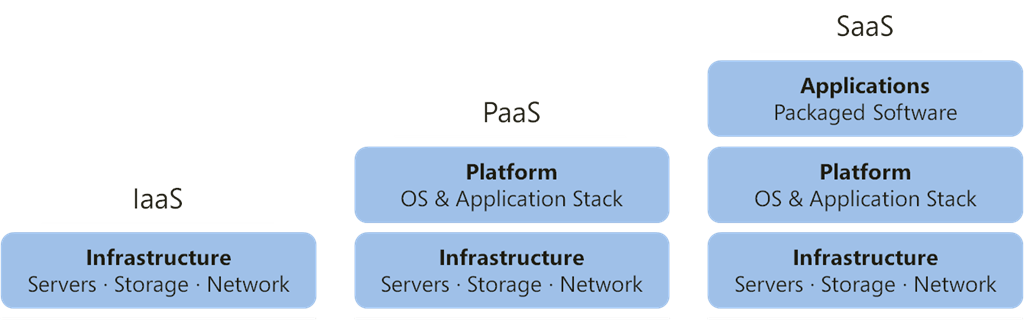
\includegraphics[width=0.6\linewidth]{resources/distributed-computing-service-models.png}
\end{figure}

\todo[inline]{Comparison in a table}
